\documentclass{article}
\usepackage[utf8]{inputenc}
\usepackage{graphicx}

\title{Driving Behavior}
\author{
Ernesto Adrián Álvarez Salazar  A00227490\\
Carlos Javier Leal Beltrán  A01741355\\
Carlos Moisés Chávez Jiménez  A01637322\\
Luis Armando Salazar López  A01114901\\
}
\date{Agosto 2022 - Septiembre 2022}

\usepackage{listings}
\usepackage{color}

\definecolor{dkgreen}{rgb}{0,0.6,0}
\definecolor{gray}{rgb}{0.5,0.5,0.5}
\definecolor{mauve}{rgb}{0.58,0,0.82}

\lstset{frame=tb,
  language=Python,
  aboveskip=3mm,
  belowskip=3mm,
  showstringspaces=false,
  columns=flexible,
  basicstyle={\small\ttfamily},
  numbers=none,
  numberstyle=\tiny\color{gray},
  keywordstyle=\color{blue},
  commentstyle=\color{dkgreen},
  stringstyle=\color{mauve},
  breaklines=true,
  breakatwhitespace=true,
  tabsize=3
}

\begin{document}

\maketitle

\section{Introduction}
El comportamiento agresivo al volante es el principal factor de los accidentes detráfico. Según informa la Fundación AAA para la Seguridad Vial, en 106.727 accidentes mortales -el 55,7% del total- durante un periodo reciente de cuatro años estuvieron implicados conductores que cometieron una o más acciones de conducción agresiva. Por lo tanto, ¿cómo predecir el comportamiento peligroso al volante de forma rápida y precisa?

La conducción agresiva incluye el exceso de velocidad, las pausas repentinas y los giros bruscos a la izquierda o a la derecha. Todos estos eventos se reflejan en los datos del acelerómetro y el giroscopio. Por lo tanto, sabiendo que hoy en día casi todo el mundo posee un smartphone que tiene una gran variedad de sensores, hemos diseñado una aplicación de recopilación de datos en android basada en los sensores del acelerómetro y el giroscopio.


\section{Tratamiento Inicial de los Datos}

Para comenzar a trabajar con los datos, es necesario que pasen por un proceso de preparación que nos permita obtener la mejor parte de ellos. Este proceso se divide en tres partes: Limpieza, Transformación y Visualización. A continuación desglosaremos las partes involucradas a esta etapa:

    \subsection{Limpieza de los datos}

        La limpieza es una parte fundamental del tratamiento de la información. En esta etapa, se busca eliminar la mayor cantidad de imperfecciones que nos pudieramos llegar a encontrar. Cosas como valores faltantes, datos fuera de rango, dividir la información disponible en "entrenamiento" y "pruebas", eliminar columnas innecesarias para el análisis, etc. Estos son algunos de los comandos que utilizamos para esta etapa:
        En el caso de nuestra base de datos, no hicimos ninguna limpieza (de momento). Encontramos muchos valores atípicos en las variables relacionadas con el movimiento de los conductores (giroscopio y acelerometro), pero no los eliminamos. Al ser demasiados, puede generar que se vaya mucha información que puede ser valiosa para nuestro modelo. Aunque no hemos definido aún si los dejaremos o no, decidimos esperar hasta avanzar un poco más en nuestra manipulación de los datos. Pero lo importante, no encontramos valores faltantes, ni columnas innecesarias. \\

        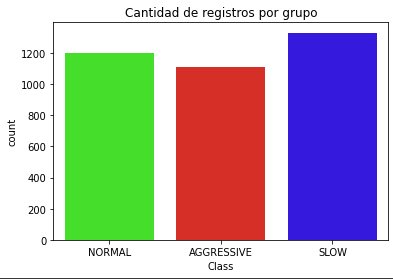
\includegraphics{images/Columnas.png} \\

        \textbf{Gráfico de barras sobre las clases disponibles en nuestro archivo de datos.} \\

    \subsection{Transformación de los datos}

        Una vez terminado el revisado de los datos, entendemos que debemos transformarlos para generar gráficos y diagramas que faciliten la busqueda de patrones y la determinación de si será necesario un modelo predictor de regresión o de clasificación.
        Para esto, revisamos el dataframe con las variables y los datos proporcionados. Encontramos que primero debemos ordenar los datos con base en el timestamp. Esta variable indica el tiempo con el que fueron realizadas las pruebas de los conductores. Se generaron dos observaciones por segundo, lo que indica que tenemos que separarlas para que queden enumeradas de uno en uno. Le restamos el primer valor del timestamp a todas las observaciones para dejar la inicial en 0, y separamos los valores para que quedaran enumeradas por el número de observación y no por el tiempo. Así no habría dos observaciones en el mismo segundo.
        Este fue el tratado que le dimos a la información previo a visualizarla. Los datos venían en buenas condiciones, por lo que no tuvimos que arreglar valores núlos, ni valores que vinieran en formatos con los que no se puede trabajar.
            

    \subsection{Visualización de los datos}

        Para la visualización de los datos es un caso diferente. Pertenece igualmente a las fases previas al trabajo de los datos, pero no involucra descartar información. La visualización involucra convertir los datos a diagramas o elementos gráficos que faciliten el entendimiento de la información. También para esta etápa consideramos el cambiar algúnas variables de tipo de dato.

        Con base en los datos que contamos para relizar este trabajo, análizamos y decidimos qué diagramas utilizar para acercarnos al desarrollo de nuestro modelo. Seleccionamos los diagramas de correlación y cajas y bigotes. \\
        El diagrama de correlación nos permite conocer qué variables son más afínes a la variable que estamos intentado predecir. Lo cual nos ahorra mucho trabajo para seleccionar las variables que estarán involucradas en nuestro modelo. \\

        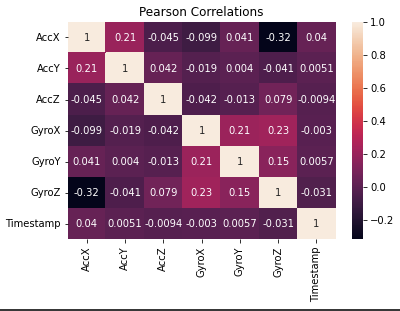
\includegraphics{images/Correlacion.png} \\

        \textbf{Gráfico de correlación entre nuestras variables.} \\
        
        El diagrama de cajas y bigotes nos permitió conocer si hay valores atípicos en nuestros datos con respecto a las variables independientes. De esta forma nosotros podemos descartar estos valores para hacer un modelo más ajustado y apegado a la realidad. Pero, para este caso particular, no debemos hacerlo. Al ser tantos este tipo de valores, el eliminarlos podría maquillar los datos y generar un modelo erroneo.\\

        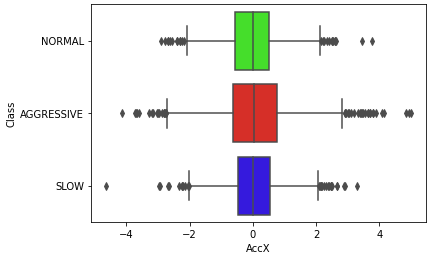
\includegraphics{images/Cajas y Bigotes AccX.png} \\

        \textbf{Gráfico de cajas y bigotes sobre la variable de aceleración "Acc X".} \\

\section{Desarrollo del modelo con los datos}

Habiendo trabajado ya con las primeras partes de los datos, ya podemos sacar conclusiones en cuanto a los patrones que buscamos, el cómo vamos a trabajar con los datos, cuántos datos requerimos para predecir y qué modelo elegir. A este punto, ya podemos definir la hipotesis que buscamos comprobar con nuestro modelo. 

    \textbf{Hipotesis Nula: Se puede predecir el comportamiento y el peligro de un conductor con base en observaciones de tipos sobre su conducción: los cambios en la aceleración total (suma de las aceleraciones en las tres dimensiones) y los cambios en el giro total (suma del giro en las tres dimensiones).} \\
        
    \subsection{Busqueda de patrones}

        La visualización nos permitió entender que no estamos buscando un modelo nos prediga una clase con base a los parametros, sino un conjunto de observaciones que nos permita clasificar el tipo de conductor con base en la información de como conduce. Al momento de análizar los gráficos que obtuvimos de los datos, encontramos algunos comportamientos y patrones que nos pueden acercar al desarrollo del modelo. Vimos que el comportamiento del conductor agresivo es cambiante constantemente y extremo en cuanto a los cambios de aceleración y direccion en todas las direcciones. Para comprobar esto, sacamos el valor vectorial de las tres dimensiones de la aceleración y el giro para generar un grafico que nos permita comprobar nuestra hipotesis.

        \includegraphics{images/Aceleración Total.png} \\

        \textbf{Gráfico de Lineas sobre la suma de las aceleraciones en las tres dimensiones del acelerómetro.} \\

        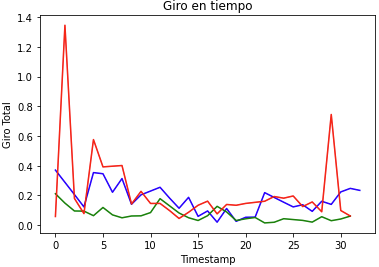
\includegraphics{images/Giro Total.png} \\

        \textbf{Gráfico de Lineas sobre la suma del giro en las tres dimensiones del giroscopio.} \\

        Como vimos en los anteriores gráficos, notamos que los valores del conductor agresivo se disparan y cambian constantemente. Esto simplemente nos muestra que nuestra hipotesis en cuanto a la inestabilidad y capacidad de predicción con base en los cambios de aceleración y el giro se comprueba. Esto nos da una idea de lo que buscamos en nuestro modelo, y nos da una pauta de lo que podemos hacer para generar un modelo eficiente.

    \subsection{Desarrollo del modelo}

        Para comenzar el desarrollo es necesario primero definir si sera de regresión o de clasificación. Este será de clasificación, nosotros esperamos recibir determinada cantidad de observaciones tomadas el manejo de un conductor, y determinar si qué tipo de conductor es. Teniendo definido esto, es importante determinar cuántas observaciones serán necesarias para que el modelo haga la predicción. Para calcular esto...

        

\end{document}
